\section{Results}
\label{sec:results}

\subsection{Measurements taken by our group}
The data that our group measured is listed in \autoref{tab:results_own} and plotted in
\autoref{fig:photocurrent_own}. While the data for $U>0$ looks similar to ???, the data points show
a linear behavior in the negative regime.

To show the linear relation ship, a function of the form
\[
  f(x; m, b) = m\cdot x + b
\]
has been fitted to the data points for $U<0$, where $m$ and $b$ are the variable fit coefficients.
To fit the function the curve\_fit from scipy.optimize has been used. It lead to the results
\begin{align}
  m &= (3.73 \pm 0.04) \, \si{\pico\ampere / \volt} \\
  b &= (299.4 \pm 0.6) \, \si{\pico\ampere}.
\end{align}
Relative uncertainty for the linear correlation is $1.1\%$, which strongly disagrees with the
expected behavior as shown in \autoref{fig:expected_curve}. The fit-function has been plotted in
\autoref{fig:photocurrent_own} as well.

% Results from our measurement
\begin{table*}
  \centering
  \caption{Results from self-performed measurement for each run. Computed values for
    average, standart deviation and relative
  uncertainty. For the first run there are no results for $U\geq\SI{28}{V}$ because of human error.}
  \label{tab:results_own}
  \sisetup{table-format=2.1}
  \begin{tabular}{c c c c c c c}
    $U / \si{V}$ &
    $I / \si{pA}$ \nth{1} run &
    $I / \si{pA}$ \nth{2} run &
    $I / \si{pA}$ \nth{3} run &
    $\overline{I} / \si{pA}$ &
    $\sigma_I / \si{pA}$ &
    $\sigma_I / \overline{I}$ \\
    \hline
    -30&201  &191&162&184.67&16.54&8.96\% \\
    -29&205  &194&167&188.67&15.97&8.46\% \\
    -28&211  &199&171&193.67&16.76&8.65\% \\
    -27&216  &203&174&197.67&17.56&8.88\% \\
    -26&220  &206&178&201.33&17.46&8.67\% \\
    -25&224  &212&183&206.33&17.21&8.34\% \\
    -24&227  &214&187&209.33&16.66&7.96\% \\
    -23&231  &218&191&213.33&16.66&7.81\% \\
    -22&236  &224&195&218.33&17.21&7.88\% \\
    -21&240  &226&200&222.00&16.57&7.47\% \\
    -20&243  &229&203&225.00&16.57&7.37\% \\
    -19&246  &233&208&229.00&15.77&6.89\% \\
    -18&250  &238&212&233.33&15.86&6.80\% \\
    -17&255  &243&216&238.00&16.31&6.85\% \\
    -16&257  &246&220&241.00&15.51&6.44\% \\
    -15&262  &250&224&245.33&15.86&6.46\% \\
    -14&266  &253&228&249.00&15.77&6.33\% \\
    -13&268  &259&232&253.00&15.30&6.05\% \\
    -12&271  &261&238&256.67&13.82&5.38\% \\
    -11&275  &266&241&260.67&14.38&5.52\% \\
    -10&278  &267&244&263.00&14.17&5.39\% \\
    -9&282   &271&249&267.33&13.72&5.13\% \\
    -8&285   &276&253&271.33&13.47&4.97\% \\
    -7&288   &277&255&273.33&13.72&5.02\% \\
    -6&291   &279&260&276.67&12.76&4.61\% \\
    -5&294   &284&263&280.33&12.92&4.61\% \\
    -4&296   &287&265&282.67&13.02&4.61\% \\
    -3&299   &289&267&285.00&13.37&4.69\% \\
    -2&301   &292&271&288.00&12.57&4.36\% \\
    -1&305   &297&275&292.33&12.68&4.34\% \\
    -0.01&315   &304&282&300.33&13.72&4.57\% \\
    0.01&307    &299&282&296.00&10.42&3.52\% \\
    1&333    &318&300&317.00&13.49&4.26\% \\
    2&360    &350&333&347.67&11.15&3.21\% \\
    3&379    &374&360&371.00&8.04&2.17\% \\
    4&396    &394&379&389.67&7.59&1.95\% \\
    5&409    &405&396&403.33&5.44&1.35\% \\
    6&420    &416&411&415.67&3.68&0.89\% \\
    7&430    &430&423&427.67&3.30&0.77\% \\
    8&440    &439&434&437.67&2.62&0.60\% \\
    9&449    &445&443&445.67&2.49&0.56\% \\
    10&457   &453&451&453.67&2.49&0.55\% \\
    11&463   &460&460&461.00&1.41&0.31\% \\
    12&471   &465&470&468.67&2.62&0.56\% \\
    13&480   &470&471&473.67&4.50&0.95\% \\
    14&483   &476&478&479.00&2.94&0.61\% \\
    15&486   &483&482&483.67&1.70&0.35\% \\
    16&491   &487&483&487.00&3.27&0.67\% \\
    17&493   &490&487&490.00&2.45&0.50\% \\
    18&496   &491&492&493.00&2.16&0.44\% \\
    19&500   &490&497&495.67&4.19&0.85\% \\
    20&507   &493&497&499.00&5.89&1.18\% \\
    21&509   &495&499&501.00&5.89&1.18\% \\
    22&512   &497&501&503.33&6.34&1.26\% \\
    23&513   &500&505&506.00&5.35&1.06\% \\
    24&509   &500&508&505.67&4.03&0.80\% \\
    25&512   &502&511&508.33&4.50&0.88\% \\
    26&513   &504&513&510.00&4.24&0.83\% \\
    27&516   &505&514&511.67&4.78&0.94\% \\
    28&&506&515&510.50&4.50&0.88\% \\
    29&&510&518&514.00&4.00&0.78\% \\
    30&&512&519&515.50&3.50&0.68\% \\
  \end{tabular}
\end{table*}


\begin{figure*}
  \centering
  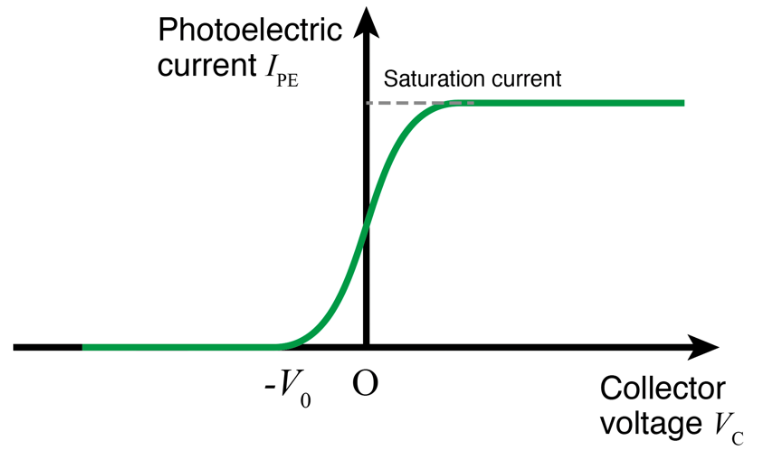
\includegraphics{build/photocurrent.pdf}
  \caption{Photo current for varying external voltages between sample and collector. Measurements taken by 
  our own group are plotted in black, note the linear relation between current and voltage for
  $U<0$. The data given to us by the TA is plotted in blue without uncertainties.}
  \label{fig:photocurrent}
\end{figure*}
